\documentclass{article}

\usepackage[pdftex]{graphicx}
\usepackage{siunitx}

% *** CITATION PACKAGES ***
%
\usepackage{cite}
% cite.sty was written by Donald Arseneau
% V1.6 and later of IEEEtran pre-defines the format of the cite.sty package
% \cite{} output to follow that of the IEEE. Loading the cite package will
% result in citation numbers being automatically sorted and properly
% "compressed/ranged". e.g., [1], [9], [2], [7], [5], [6] without using
% cite.sty will become [1], [2], [5]--[7], [9] using cite.sty. cite.sty's
% \cite will automatically add leading space, if needed. Use cite.sty's
% noadjust option (cite.sty V3.8 and later) if you want to turn this off
% such as if a citation ever needs to be enclosed in parenthesis.
% cite.sty is already installed on most LaTeX systems. Be sure and use
% version 5.0 (2009-03-20) and later if using hyperref.sty.
% The latest version can be obtained at:
% http://www.ctan.org/pkg/cite
% The documentation is contained in the cite.sty file itself.

\usepackage{booktabs}
\usepackage{lscape}
\usepackage{svg}

% *** MATH PACKAGES ***
%
\usepackage{amsmath}
% A popular package from the American Mathematical Society that provides
% many useful and powerful commands for dealing with mathematics.
%
% Note that the amsmath package sets \interdisplaylinepenalty to 10000
% thus preventing page breaks from occurring within multiline equations. Use:
\interdisplaylinepenalty=2500
% after loading amsmath to restore such page breaks as IEEEtran.cls normally
% does. amsmath.sty is already installed on most LaTeX systems. The latest
% version and documentation can be obtained at:
% http://www.ctan.org/pkg/amsmath



% correct bad hyphenation here
\hyphenation{op-tical net-works semi-conduc-tor}

%\usepackage[utf8]{inputenc}
%\usepackage{helvet}
%\usepackage[usenames,dvipsnames,svgnames,table]{xcolor}
%\usepackage{graphicx}
%\usepackage{caption}
%\usepackage{subcaption}
%\usepackage{url}
%\usepackage{amstext}
% \usepackage{booktabs}

%\bibliographystyle{IEEEtran}

% Title Page
\title{Mapping Deforestation with Recurrence Metrics of Sentinel-1 time series}
\author{Felix Cremer, Mikhail Urbazaev, Christiane Schmullius and Christian Thiel}

%\IEEEauthorblockA{Chair of Earth Observation, Friedrich-Schiller University, Jena,Germany\\
%Email: felix.cremer@uni-jena.de}

\begin{document}
\maketitle
%\tableofcontents
\begin{abstract}
  Forest ecosystems
  REDD+ process
  order of time series
  SAR

%Keywords:Recurrence, SAR, time series, remote sensing
%
\end{abstract}
\section{Introduction}
The tropical forest ecosystems stabilise the world climate\cite{}, the protection of the biodiversity \cite{} and
for the well being of a vast amount of the global popu-
lation\cite{}.
 In the last decade remote sensing technologies have
played a substantial role in the consistent, reliable and timely
information gathering about forest cover changes. With the
REDD+ mechanism the use of remote sensing to monitor
and map deforestation and degradation processes increased.
Forest/Non-Forest maps are mostly operationally if
they are based on optical sensors. Especially in the tropics,
the optical imaging is hindered by clouds. In this study we
 propose a deforestation mapping approach based on SAR time
series.

Established method to map forest cover change from optical images using Landsat \cite{Hansen}.
Optical satellite data acquisitions is hindered by clouds, which is especially problematic in the tropics.
Therefore there has been some research going into the mapping of forest cover change using synthetic aperture radar data.
The detection of deforestation is better with the use of L-Band data, because the higher wavelengths better distinguishes between the forest cover and bare soil.
Unfortunately, there are no global L-Band products freely available.
For C-Band, there is a global dataset with a high temporal repetition available thanks to the european Sentinel-1 mission.
The separabiltiy between the forest cover and the bare soil in C-Band data can be enhanced by the use of the full time series.


Misses overview about established methods.
Especially the percentile range

\section{Method}

\subsection{Recurrence Plots}

Recurrence plots (RP) have been proposed by Eckmann et al 1987. They are a method to visualize the recurrences of a time series.
They are defined as follows:
$$R_{i,j} = \theta(\epsilon - \lvert x_i - x_j \rvert), i,j = 1,...,N$$
hereby $\epsilon$ is a threshold value which indicates up to which distance two time steps are viewed as similar.
$\theta$ is the Heaviside function which sets everything below zero to zero and every positive value to one.
N is the number of time steps.
This leads to a quadratic matrix with black dots where the time steps are similar to each other and white dots where they are distinct.
The main diagonal is always black, because every time step is similar to itself.
It is a nonlinear data analysis tool.
Figure \ref{rplots} shows example Recurrence plots of a sum of two sine waves with different frequencies,
a step function from three to zero with an overlaid white noise with standard deviation 1 and third a sine wave with overlaying trend.
For the composition of two different frequencies we can see a regular pattern with distinguished diagonals which are indicating the frequency.
In the noisy step function we see four distinct quadrants in the recurence plot.
In the two quadrants near the main diagonal every point is randomly similar to other points in this part of the time series with a high probability.
In the other two quadrants, the probability is low, that two points are similar to a point in the other part of the step function.
In the third example, we see a clear pattern, but these patterns are fading out to the edge of the recurrence plot.
This is due to the difference of the values at the beginning and the end of the time series.
Therefore we can use this pattern as an indicator for a trend in the time series.

\begin{figure}
  \includegraphics[width=\textwidth]{figs/rp_methods.png}
  \caption{Recurrence Plots for a sine wave, a step function with noise, and a sine wave with trend.}
  \label{rplots}
\end{figure}

These visual patterns can be quantified using recurrence quantification analysis (RQA)\cite{Zbilut}.
The simplest measure is the recurrence rate (RR) which is the number of recurrences in a recurrence plot devided by the squared number of time steps.
It measures the density of the recurrence points in a RP.
Another measure is the trend.
It is defined as
$$ TREND= \frac{\sum_{\tau=1}^{\tilde{N}}(\tau - \tilde{N}/2)(RR_\tau - \langle RR_\tau \rangle)}{\sum_{\tau=1}^{\tilde{N}}(\tau - \tilde{N}/2)}.$$
It is a linear regression coefficient over the recurrence rate of the diagonals in comparison to their distance to the main diagonal.
It indicates if the process is drifting.
For an overview of RQA measures see  Table \ref{RQA_table} and for an in depth discussion \cite{Marwan06}.
All of the results have been produced using the Julia RecurrenceAnalysis.jl package\cite{RQA.jl}.

\begin{landscape}
\renewcommand{\arraystretch}{2}
\begin{table}[]
\centering
\begin{tabular}{p{3cm}p{4cm}p{14cm}}
\toprule
 Name & Formula & Interpretation \\
 \midrule
 Recurrence Rate & $\frac{\sum\limits_{i,j=1}^N(R_{i,j})}{N^2} $ & Probability that a state of the system recurs.  \\
 Determinism & $\frac{\sum\limits_{l=lmin}^N(l P(l))}{\sum_{l=1}(l P(l))} $ & Measures the predictability of the signal.   \\
 Average Length \newline of Diagonal Structues & $\frac{\sum_{l=lmin}(l P(l))}{\sum_{l=lmin}^{N}(P(l))}$  &  \\
 Maximum Length \newline of Diagonal Structures & $\max(l_i)$ &  \\
 Divergence & $\frac{1}{\max(l_i)}$ &  \\
 Entropy of diagonal structures & $\sum\limits_{i=1}^N P(l_i) * log(P(l_i))$ & Indicates the complexity of the diagonal line structure of the RP, small for uncorrelated noise  \\
 Trend & $ \frac{\sum_{\tau=1}^{\tilde{N}}(\tau - \tilde{N}/2)(RR_\tau - \langle RR_\tau \rangle)}{\sum_{\tau=1}^{\tilde{N}}(\tau - \tilde{N}/2)}$ &
  Linear regression between the recurrences on a diagonal and the distance to the main diagonal. Normal distributed around zero.
   Low values indicate, that time steps that are further apart are more seldom similar \\
 Laminarity & $\frac{\sum_{v=vmin}(v P(v))}{\sum_{v=1}^{N}(v P(v))}$ &  \\
 Trapping time & $\frac{\sum_{v=vmin}(v P(v))}{\sum_{v=vmin}^{N}(P(v))}$ &  \\
 Maximum Length of vertical structures & $\max\limits_{i=1, ..., N}(v_i)$ &  \\
 Entropy of vertical structures& $\sum\limits_{i=1}^N P(v_i) * log(P(v_i))$ &  \\
 Mean recurrence time & $\frac{\sum\limits_{i=1}^N(w_i P(w_i))}{\sum_{1}^{N}(P(w_i))}$  &  \\
 Recurrence time entropy & $\sum\limits_{i=1}^N P(w_i) * log(P(w_i))$  & \\
 Number of the most probable recurrence times & $\max w_i$ & \\ \bottomrule
\end{tabular}
\caption{Overview of Recurrence Quantification measures.}
\label{RQA_table}
\end{table}
\end{landscape}

\section{Experimental Results}
\subsection{Data and Preprocessing}
We test the separability of stable forest and deforestation on two testsites in Mexico.
One is mostly covered by temperate forests in central Mexico,
the other is situated on the Yucatan peninsula and is covered by tropical dry forests.
Figure \ref{testsites} show very high resolution Pléiades data of the two testsites.

\begin{figure}
  \includegraphics[width=\textwidth]{figs/SEN4REDD_testsites.png}
  \caption{The testsites are located in Mexico and are dominated by temperate forests (Hidalgo) and tropical dry forest(Kiuic).}
  \label{testsites}
\end{figure}

The data have been preprocessed using the SNAP software \cite{SNAP} in version 6.
The single time steps are multilooked to a \SI{10}{\m} x \SI{10}{\m} pixel spacing.
The orthorectification is based on the original orbit state vectors and the \SI{30}{\m} SRTM digital elevation model\cite{SRTM}.
The preprocessing also included radiometric terrain flattening after \cite{Small} which results in $\gamma^0$ backscatter values.
All images were coregistered in the DEM geometry after geocoding to achieve a subpixel coregistration precision which is of eminent importance when the pixels are investigated in the temporal domain only.
We used the python package pyroSAR \cite{pyroSAR} to handle the preprocessing.

We have reduced the speckle noise and other unwanted short-term perturbations of the data using the filter described in \cite{Cremer2018}.
The filter is based on the Empirical Mode Decomposition a data adaptive alternative to the fourier transformation which can handle non-stationary data.
Each pixel is separately decomposed into intrinsic mode functions (IMFs) of different temporal frequencies.
In order to reduce the speckle, the two IMFs with the highest temporal frequencies are removed.
This results in a nonparametric image transform that fully preserves the geometric resolution and has a similar speckle suppression than the Quegan 5x5 filter \cite{Quegan_2001}.


\subsection{Separability analysis}

Figure \ref{rpforest} shows the recurrence plots of a neighbourhood of examplary forest and deforestation areas.
The upper figures shows the cross-pol time series of a 7x7 matrix of a deforested area (left) and a stable forest (right) with the mean of these pixels in red respectively green.
The bottom figures show the grayscale of the corresponding recurrence plots.
Black points are similar in every pixel of the neighborhood and white points in none.
There is a clear drop in the backscatter time series of the deforested area, but then the signal is going up to a similar level than before the deforestation.
In the Recurrence Plot this change is visible as large white areas in the corners of the recurrence plots similar to the second example in Figure \ref{rplots}.
In the forest, the signal is stable with small backscatter differences between every time step. This is visible in the recurrence plot as a white noise.

\begin{figure}
  \includegraphics[width=\textwidth]{figs/S1_Hidalgo_timestack_20km_VH___lin_20_test_tandemdem12_emd__rp_deffor_3.png}
  \caption{Recurrence Plots for a 7x7 matrix of deforestated(left) and stable forest(right) pixels.
           The gray lines in the above figure are all pixels and the colored line is the mean of these pixels.}
  \label{rpforest}
\end{figure}

Figure \ref{trend} shows the RQA TREND statistic from two year VH data from march 2017 till march 2019 in comparison to the range between the multitemporal 5th to 95th percentile (prange).
For this time frame are 187 time steps available.
The red polygons are deforestations which happened between september 2016 and october 2017 and the violet ones deforestations between October 2017 and July 2018.
The later deforestations which are fully in our sensing period are distinctly visible as clear black areas in the RQA TREND metric.
The EMD filter reduces the pixel inside the deforestation areas which are having a low RQA TREND metric especially in the left polygon in VV data.
In the prange metric from the original data is no clear difference visible between the deforested areas and the surrounding stable forest areas.
Applying the EMD filter makes the deforestations visible.
The earlier deforestations are also partly visible, because the deforestations happened in the beginning of the sensing period.
Therefore the 95th percentile is from the still standing forest and the 5th percentile is dominated by the already deforested signal.
The prange metric gains especially from the temporal denoising by the EMD filter.
Overall is the cross-pol data better suited to map deforestations than co-pol data.
Therefore, we are only showing the cross-pol results hereafter.


\begin{figure}
  \includegraphics[width=\textwidth]{figs/rqa_trend_0317_0319.png}
  \caption{RQA TREND statistic.  The red polygons are deforestations between October 2017 and July 2018 and the green polygons are stable forest areas.
  These polygons have been select from VHR Pleiades data.}
  \label{trend}
\end{figure}


\begin{figure}
  \includegraphics[width=\textwidth]{figs/comp_vh_a_d_def.pdf}
  \caption{Recurrence Plots for a 7x7 matrix of deforested pixels in ascending(left) and descending(right) orbit.
           The gray lines in the above figure are all pixels and the colored line is the mean of these pixels.}
  \label{rpdef_a_d}
\end{figure}

Figure \ref{ts_a_d} shows the VH time series of a 7x7 matrix of deforested pixels in the ascending and descending orbit.
Figure \ref{rpdef_a_d} shows these time series with the corresponding recurrence plots.
The ascending time series have a little bit higher values while it is still forested
and have a little bit lower values after the deforestation.
Since the threshold for similarity in the recurrence plots is 1.5 dB,
there are more timesteps in the descending orbit, which are classified as similar.
Therefore, are the recurrence plots from the ascending orbit showing a clearer distinguishable whitespace at the time of the deforestation.
The differences between the number of time steps before the deforestation is due to a lack of data in the ascending orbit from september 2017 to january 2018.
This does not have an effect on the computation of the rqa trend metric.
The differences in the recurrence plots have also an impact on the rqa trend metric as we can see in figure \ref{comp_vh_a_d}.




\begin{figure}
  \includegraphics[width=\textwidth]{figs/vh_a_d_timeseries.pdf}
  \caption{Cross polarisation time series of 7x7 deforested pixels for the ascending and descending stack.
            The ascending data has a higher variance and a higher difference between before and after the deforestation.
            }
  \label{ts_a_d}
\end{figure}

\begin{figure}
  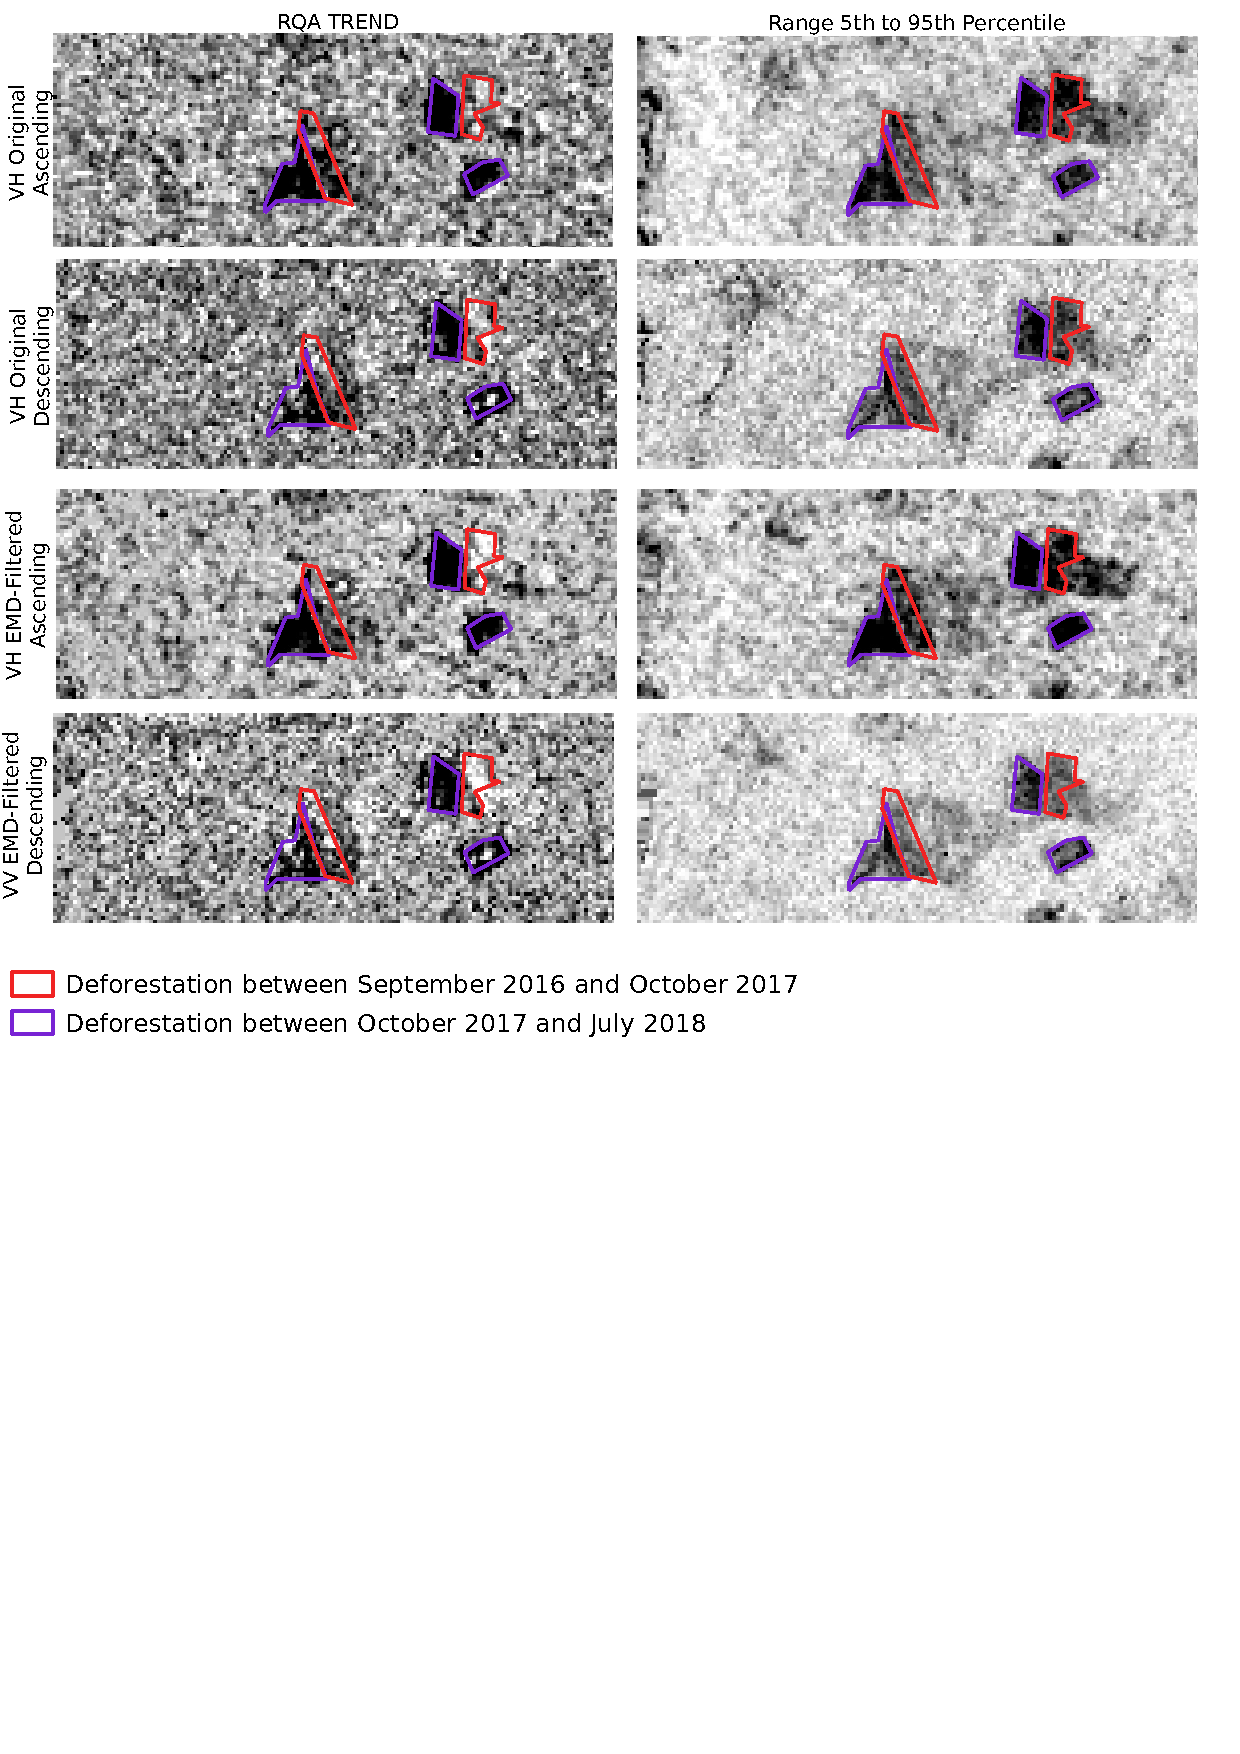
\includegraphics[width=\textwidth]{figs/rqa_trend_vh_a_d_comp.pdf}
  \caption{Comparison of the RQA trend metric and the percentile range for the cross-pol time series in the ascending and descending orbit.The ascending orbit is better suited to map deforestations.}
  \label{comp_vh_a_d}
\end{figure}

\subsection{Histogram analysis}

Figure \ref{histtrend} shows the histograms for the RQA trend metric and figure \ref{histprange} the ones for the percentile range for the deforestation areas in red and the stable forest areas in green.

\begin{figure}
  \includegraphics[width=\textwidth]{figs/histogram_trend1_5_0317_0319_polygon_5.png}
  \caption{Histogram of the RQA Trend metrics for a deforestation(red) and a stable forest area (green) of similar size.}
  \label{histtrend}
\end{figure}


\begin{figure}
  \includegraphics[width=\textwidth]{figs/histogram_percrange_0317_0319_polygon_5.png}
  \caption{Histogram of the prange for deforestation(red) and stable forest areas (green) of similar size.}
  \label{histprange}
\end{figure}

Check wether the histograms are VH or VV I suppose, they are VH

Show that the TREND metric is enhancing the separability of deforested areas and stable forests.

Quantify it.


Is there a recommendation, which threshold we should use for the percentile range?

\section{Discussion}

discuss the differences between EMD filtered and original data

discuss the differences between asc and desc

Remarks about the water content.


difference between prange and rqa trend



\section{Summary and Conclusion}
In this work, we showed, that the RQA TREND metric is a good indicator for deforestations.
We compared the RQA TREND to the range between the 5th and the 95th multitemporal percentile.
Because the RQA TREND is also using the order of the time series to derive information about the underlying land cover,
it gives a clearer picture about deforestations.



\section*{Acknowledgment}
This work was funded by the DLR in the Sentinel4REDD project (FKZ:50EE1540) and
the DFG project HyperSense.
This work uses Copernicus Sentinel data 2017-2019.


\bibliographystyle{ieeetr}
\bibliography{literatur}

\end{document}
